%%%%%%%%%%%%%%%%%%%%%%%%%%%%%%%%%%%%%%%%%%%%%%%%%%%%%%%%%%%%%%%%%%%%%%%%%%%%%%%%
%2345678901234567890123456789012345678901234567890123456789012345678901234567890
%        1         2         3         4         5         6         7         8

\documentclass[letterpaper, 9pt, conference]{ieeeconf}  % Comment this line out
                                                          % if you need a4paper
%\documentclass[a4paper, 10pt, conference]{ieeeconf}      % Use this line for a4
                                                          % paper

\IEEEoverridecommandlockouts                              % This command is only
                                                          % needed if you want to
                                                          % use the \thanks command
\overrideIEEEmargins
% See the \addtolength command later in the file to balance the column lengths
% on the last page of the document



% The following packages can be found on http:\\www.ctan.org
\usepackage{graphics} % for pdf, bitmapped graphics files
%\usepackage{epsfig} % for postscript graphics files
\usepackage{mathptmx} % assumes new font selection scheme installed
\usepackage{times} % assumes new font selection scheme installed
\usepackage{amsmath} % assumes amsmath package installed
\usepackage{amssymb}  % assumes amsmath package installed
\usepackage{graphicx}
%\usepackage{caption}
\newcommand\numberthis{\addtocounter{equation}{1}\tag{\theequation}}

\title{\LARGE \bf
Modeling Conflict between Patrilineal Clans
}

\author{SCUDEM III Fall 2018 Executive Summary}

\begin{document}



\maketitle
\thispagestyle{empty}
\pagestyle{empty}

\section{INTRODUCTION}

Given the hypotheses that around 7,000 years ago patrilineal clans formed causing a high death rate of males through conflict, we model the resulting distribution between males and females for a given number of clans\cite{problem}.

\section{Assumptions}

To simplify the process of modeling, we made some reasonable simplifying assumptions based on typical human behaviour after the first agricultural revolution.
\begin{itemize}
    \item Clans form cities that grow radially and do not move. There will be no migration of clans; there is no accounting for clans merging or forming.
    \item Resources (food, water, etc.) are evenly distributed among land, and all land is equally viable for farming. 
    %Each square unit of land supports a given number of people. Going off the guideline that about %1.2 acres is needed to support one person per year\cite{farm}, each sq. km can support about %200 people.
    \item The Earth is an infinite plane, but we only model clans with centers in a specified square area.
\end{itemize}

\section{Mathematical Model}

\subsection{Definition of a clan}
Each clan will have a position $(x,y)$ in the defined square and an initial population $P_{0,i}$ that is evenly split between males and females.

\subsection{Population Growth}
A main goal of the model is to show the dynamics of gender distribution for each clan going through conflict. We start by saying the total rate of change for a population is the sum of the rate of change of the males $dM/dt$ and females $dF/dt$.
\begin{equation}
\frac{dP_i}{dt} = \frac{dM_i}{dt} + \frac{dF_i}{dt} \label{eq:1}
\end{equation}

Looking at a typical differential equation for a population $P(t)$, $\dfrac{dP}{dt} = rP\left(1 - \dfrac{P}{K}\right)$ gives a population curve that follows a logistic function starting at initial population $P_0$ with an upper bound carrying capacity of $K$. Given that the observed land is square with side length $d$ and each $\text{km}^2$ supports $c$ people, we can define the carrying capacity of each clan as the total carrying capacity of the square as shown in (\ref{eq:2}).
\begin{equation}
    K_{net} = c\;d^2 \label{eq:2}
\end{equation}

The $r$ in the differential equation represents some type of growth rate. We define growth rate as a function of gender ratio for each clan. 
We define $ r: [0, 1] \to \mathbb{R} $ in a manner that supports no growth with a completely single-gender population and peak rate where there more females than males. An easy to evaluate function that supports these goals is shown in (\ref{eq:3}) and (\ref{eq:4}).
\begin{equation}
    r(s_i) = -s_i^3 \ln{(s_i)} \label{eq:3}
\end{equation}
\begin{equation}
    s_i(t) = \frac{F_i(t)}{P_i (t)} = \frac{F_i(t)}{F_i(t)+M_i(t)} \label{eq:4}
\end{equation}

We can finalize the growth part of the model for both males and females as below since all births will be split between the genders:

\begin{equation}
    \frac{dM_i}{dt}^{+} = \frac{dF_i}{dt}^{+} = \frac{1}{2}r(s_i)\;P_i(t)\left(1 - \frac{P_i(t)}{K_{net}}\right) \label{eq:5}
\end{equation}

\subsection{Population Decay}

We will define a specific clan's discontent, or desire to expand, $\Delta_i$ as the difference between carrying capacity and current population.
\begin{equation}
    \Delta_i = K_{net} - P_i(t) \label{eq:6}
\end{equation}

When two clans $i$ and $j$ are in sufficient contact and there is ample individual discontent, conflict arises as given in \label{eq:7} where $p$ is a possible tuning parameter for hostility between clans.
\begin{equation}
    A_{i, j} = \left(\frac{\lambda_{i, j}}{\ln(\Delta_i\Delta_j)}\right)^p \label{eq:7}
\end{equation}

To measure sufficient contact, $\lambda_{i, j}$ can have multiple definitions; we will evaluate it as shared area between clans $i, j$. We assumed earlier each clan maintains a circle proportional to population. With both radii and clan centers known, the overlapping area can be calculated.
 \cite{circle_area} The radii can be calculated as show in (\ref{eq:8}).
\begin{equation}
    P_i = cA = c \pi r_i^2 \; \Rightarrow \; r_i = \sqrt{\dfrac{P_i}{c\pi}} \label{eq:8}
\end{equation}

Finally, the total rate of change for death of males and females can be defined based on the hypotheses that males die at a much higher rate from conflict than females. We now have final versions of a differential equation where $g \in [0,1] $ represents the percent of deaths from conflict that are male. Each equation only needs to be evaluated if there are currently males and females to avoid these values becoming negative, and we will account for natural death with some factor $\eta \in \left[-1, 0\right)$ which will determine the rate of decay when reproduction is not possible; this represents the case where only one gender left in a clan (usually females). Thus, the differential equations defining the operation of our model are defined in (\ref{eq:10}) and (\ref{eq:11}).


\begin{align*}
    \frac{dM_i}{dt} 
    & =\begin{cases} 
        \dfrac{dM_i}{dt}^{+} + \dfrac{dM_i}{dt}^{-}, & \; F_i > 0 \\
        \eta M_i, & \; F_i \leq 0 \\
    \end{cases} \\
    & = \begin{cases}
        \dfrac{1}{2}r(s_i)P_i\left(1 - \dfrac{P_i}{K_{net}}\right) - g\displaystyle\sum\limits_{j \neq i} A_{i,j}, & F_i > 0 \\
        \eta M_i, & F_i \leq 0 % \\https://www.overleaf.com/project/5bce74f725621d76a6ce0458
    \end{cases} \numberthis \label{eq:10}\\
    \;\\
    \frac{dF_i}{dt}
    & =\begin{cases} 
        \dfrac{dF_i}{dt}^{+} + \dfrac{dF_i}{dt}^{-}, & \; M_i > 0 \\
        \eta F_i, & \; M_i \leq 0 \\
    \end{cases} \\
    & = \begin{cases}
        \dfrac{1}{2}r(s_i)P_i\left(1 - \dfrac{P_i}{K_{net}}\right) - \left(1-g\right)\displaystyle\sum\limits_{j \neq i} A_{i,j}, & M_i > 0 \\
        \eta F_i, & M_i \leq 0 \\
    \end{cases}
    \numberthis \label{eq:11}
\end{align*}



\section{SIMULATIONS}
To perform simulations of the model, the Forward Euler method \cite{euler_method} was used to approximate the solution. The time step $dt$ is $0.01$ and $t = 0$. The simulation was run until $t = 700$ to approximate $7000$ years with each time step representing $10$ years.

\subsection{Choosing Model Parameters}

The initial conditions for simulating each individual clan was uniformly chosen by pseudo-randomly sampling over a range of values. A random seed was used to reproduce results. A complete list of parameter ranges and values is summarized in Table \ref{tab:parameters}.
\begin{table}[!h]
    \centering
    \begin{tabular}{|c|c|c|c|}\hline
        Parameter & Symbol & Value/Range & Selected (if Global)\\ \hline
        Dimension & $d$ & $100$ & $100$ \\ \hline
        Density & $c$ & $\left(0, 10\right)$ & $7$ \\ \hline
        Death Disparity & $g$ & $\left(0.5, 0.9\right)$ & $0.58$ \\ \hline
        Hostility & $p$ & $\left(0, 10\right)$ & $3.4$ \\ \hline
        Natural Death & $\eta$ & $\left(0, 1\right)$ & $0.7$ \\ \hline
        Clan Center & $\left(x_i, y_i\right)$ & $\left(0, d\right)$ & - \\ \hline
        Initial Population & $P_0$ & $\left(50, 100\right)$ & - \\ \hline
    \end{tabular}
    \caption{Parameters for Simulations}
    \label{tab:parameters}
\end{table}

\subsection{Results}
The model defined by the parameters in Table \ref{tab:parameters} was run first with $2$ clans as the most basic case. This produced the results visualized in Fig. \ref{fig:case_2}. The simulation was further run with $8$ clans as well. The results for $8$ clans are depicted in Fig. \ref{fig:case_m}.
\begin{figure}[!htb]
\begin{center}
\minipage{0.4\textwidth}
  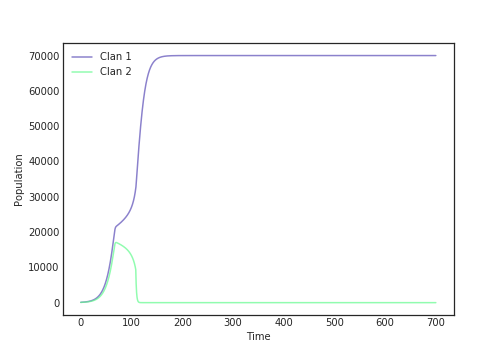
\includegraphics[width=\linewidth]{2clans_graph.png}
\endminipage\hfill
\minipage{0.15\textwidth}
  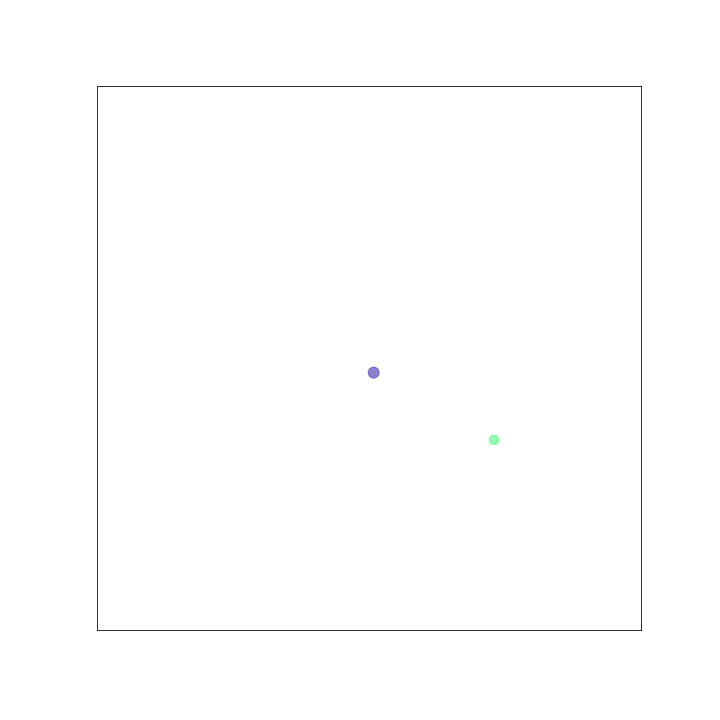
\includegraphics[width=\linewidth]{2clans_t0.png}
  \textit{\begin{center} \small $t = 0$\end{center}}
\endminipage
\minipage{0.15\textwidth}%
  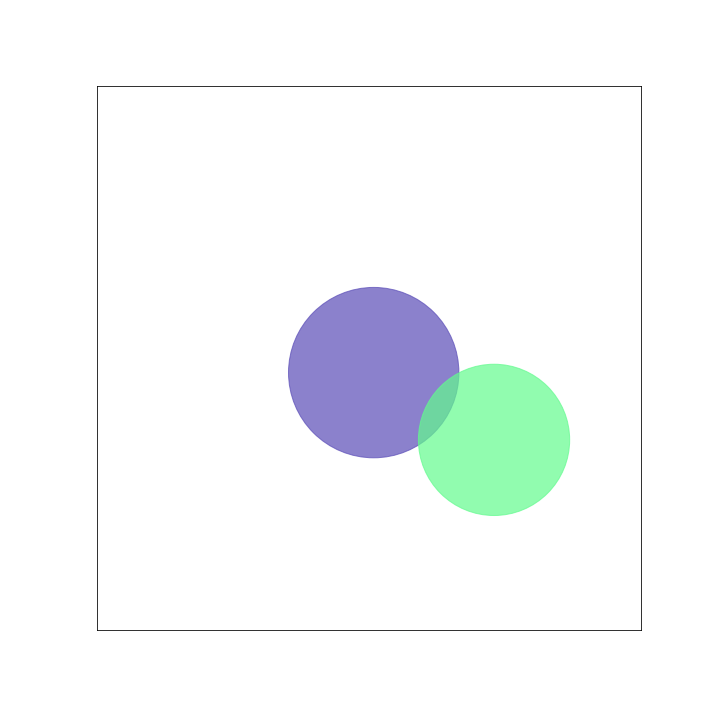
\includegraphics[width=\linewidth]{2clans_t100.png}
  \textit{\begin{center} \small $t = 100$\end{center}}
\endminipage
\minipage{0.15\textwidth}%
  
\includegraphics[width=\linewidth]{2clans_tlast.png}
  \textit{\begin{center} \small $t = 700$\end{center}}
\endminipage
\end{center}
\caption{Running the Simulation with $2$ Clans}
\label{fig:case_2}
\end{figure}


\begin{figure}[!htb]
\begin{center}
\minipage{0.4\textwidth}
  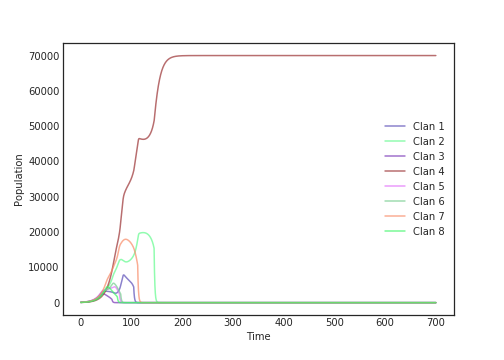
\includegraphics[width=\linewidth]{mclans_graph.png}
\endminipage\newline
\minipage{0.4\textwidth}
  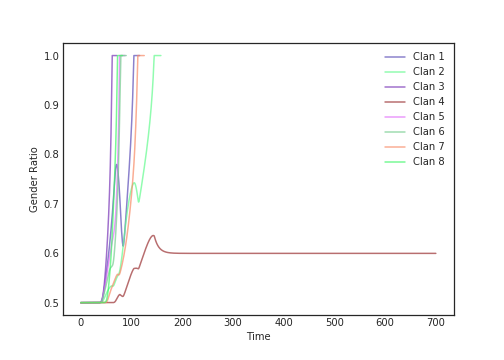
\includegraphics[width=\linewidth]{mclans_graph_s.png}
\endminipage\newline
\minipage{0.15\textwidth}
  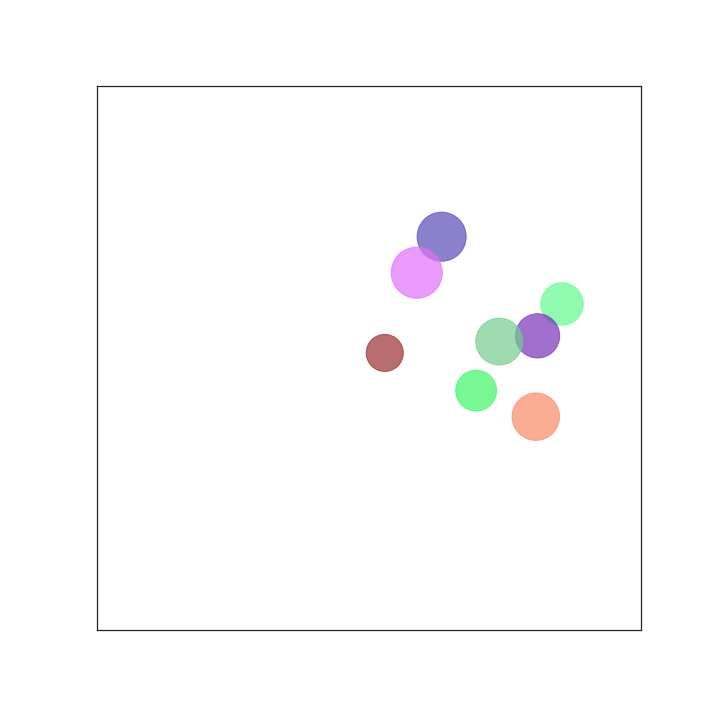
\includegraphics[width=\linewidth]{mclans_t50.png}
  \textit{\begin{center} \small $t = 50$\end{center}}
\endminipage
\minipage{0.15\textwidth}%
  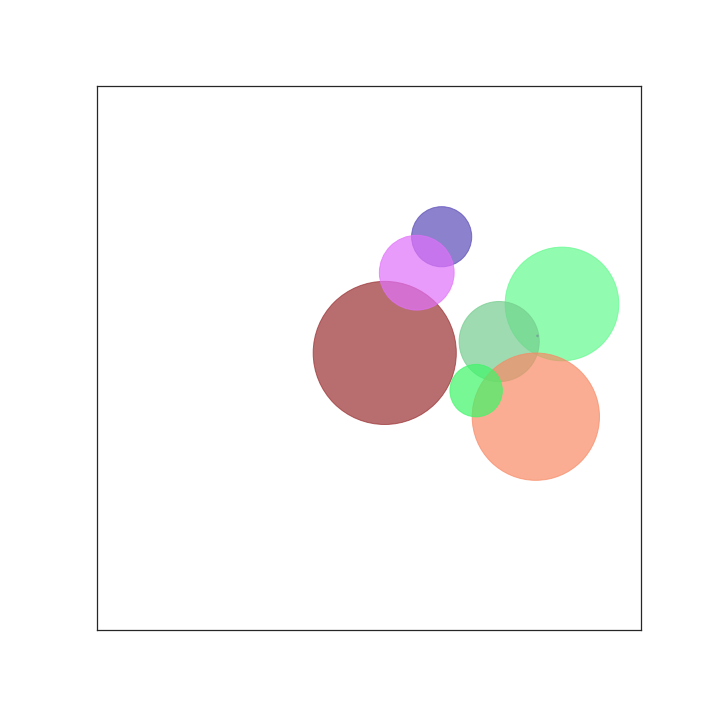
\includegraphics[width=\linewidth]{mclans_t100.png}
  \textit{\begin{center} \small $t = 100$\end{center}}
\endminipage
\minipage{0.15\textwidth}%
  
\includegraphics[width=\linewidth]{mclans_tlast.png}
  \textit{\begin{center} \small $t = 700$\end{center}}
\endminipage
\end{center}
\caption{Running the Simulation with $8$ Clans}
\label{fig:case_m}
\end{figure}


\section{CONCLUSIONS}
% Based on your models under what conditions are conflicts most intense?
The results indicate the starting distance of a clan and its neighboring clans as the main factor(s) directly affecting the amount of population decrease, or the conflict that a clan faces before reaching its carrying capacity. It is clear from Fig. \ref{fig:case_2} that the clan that is able to grow the largest the fastest tends to win conflicts versus other clans. Clan $4$ has a smaller population than Clan $7$ at $t=50$, but because it doesn't have to compete for resources, it is able to eventually able to take over by $t=200$. Equilibrium may be reached if all clans are equally spaced apart and have the same starting population, causing the patrilineal clans to maintain a small male population over time while only growing to a point that allows the birth rate to equal the death rate. Given that the world is not in uniform conditions, it is clear why patrilineal clans declined over time.

% Was the decline of patrilineal clans inevitable or is it possible to reach an equilibrium under such a social tradition?
% good good thanx bro
% yeah i was considering it, that's why i removed the t=0 for fig2
Furthermore, The decline of patrilineal clans in a restricted region is inevitable. The conflict between clans in a region will always result in a winner given some type of variation or advantage in any clan. The plot of gender ratio versus time in Fig. \ref{fig:case_m} show this clearly. The clans that die out all reach a completely single-gender population when they die out, which is a direct consequence of patrilineal conflict in a closed region.

%\clearpage
\bibliographystyle{plain}
\bibliography{biblio.bib}

\end{document}
